\documentclass[conference]{IEEEtran}
\usepackage{cite}
\usepackage{adjustbox}
\usepackage{amsmath,amssymb,amsfonts}
\usepackage{algorithmic}
\usepackage{graphicx}
\usepackage{textcomp}
\usepackage{xcolor}
\usepackage{comment}
\usepackage[table]{xcolor}
\def\BibTeX{{\rm B\kern-.05em{\sc i\kern-.025em b}\kern-.08em
    T\kern-.1667em\lower.7ex\hbox{E}\kern-.125emX}}
    
\begin{document}

\title{Project: COVID-19 Assisted Diagnosis\\

\author{\IEEEauthorblockN{Carlo Heemeryck\textsuperscript{1}}
\and
\IEEEauthorblockN{Willem Van Nieuwenhuyse\textsuperscript{1}}
\and
\IEEEauthorblockN{Seppe Vanrietvelde\textsuperscript{2}}
\and
\IEEEauthorblockN{Luca Visser\textsuperscript{2}}
\and

\textsuperscript{1} Bachelor of Science in de ingenieurswetenschappen - werktuigkunde-elektrotechniek \hfill\\
\textsuperscript{2} Master of Science in Statistical Data Analysis - Computational Statistics\hfill\\}
}
\maketitle

\section{Introduction}
The outbreak of the COVID-19 pandemic in late 2019 has placed unprecedented strain on healthcare systems worldwide, highlighting the urgent need for rapid and accurate diagnostic tools to support clinical decision–making. Chest X‑ray imaging has emerged as a widely available modality for the preliminary screening of COVID‑19 pneumonia, yet visual assessment alone can be time‑consuming and prone to inter‑observer variability~\cite{b1,b2}. In this work, a deep learning–based framework for assisted diagnosis of COVID‑19 from chest X‑ray images is presented, leveraging both custom convolutional neural networks and transfer learning approaches.

Section~\ref{sec:task_1} covers exploring the publicly available dataset, detailing the preprocessing pipeline (downsampling, normalization, and light augmentation) and presenting initial sample images (Fig.~\ref{fig:example_images}). In Section~\ref{sec:task_2}, a baseline CNN model is build and evaluated, reporting its architecture (Table~\ref{table:baseline_cnn_overview}), learning curves (Fig.~\ref{line_curves}), and test‑set performance including a confusion matrix (Fig.~\ref{fig:conf_matrix}). Section~\ref{sec:task_3} introduces transfer learning with a pre‑trained ResNet50V2 backbone, describing model adaptations, hyperparameter tuning, and comparative results. Section~\ref{sec:task_4} demonstrates model interpretability using Grad‑CAM heatmaps, and finally Section~\ref{sec:conclusions} summarizes the conclusions and outlines potential future work.

\vspace{1cm}
\section{Task 1: Data Exploration, Pre-Processing and Augmentation}\label{sec:task_1}
\subsection{Loading the data}
The grayscale chest X-ray images are loaded at their original resolution of 299 × 299 pixels. The labels, either COVID or NORMAL, are taken from the folder names containing the images and assumed to be accurate. From the outset, the dataset was pre-divided into training (1,600 images), validation (400 images), and test (200 images) sets. This original distribution is preserved for the exercise, with an additional combined training and validation set comprising 2,000 images.

\subsection{Data exploration}
Exploration consists of checking the shape of the data, evaluating the distribution of the two classes, plotting a few examples and checking pixel and global average and standard deviation. This is replicated for training, validation and test datasets and serves as an initial look at the data and to possibly detect problems at an early stage in the project.
All the images in the training dataset are of the same size and there are an equal amount in both classes, which is good. A few labeled examples are given in Fig.~\ref{fig:example_images}.

\begin{figure}[htbp]
\centerline{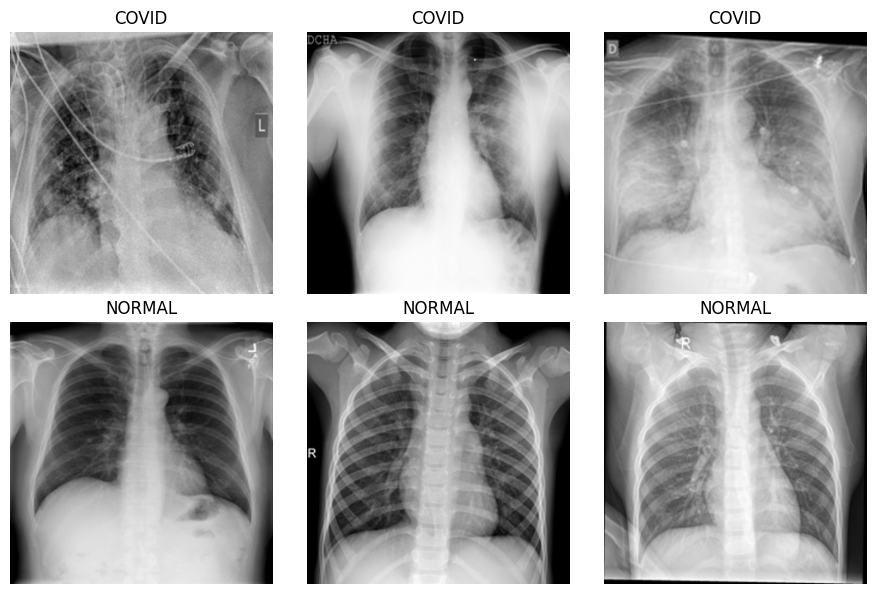
\includegraphics[width=\linewidth]{Images/example_images.png}}
\caption{A few images from the training dataset with accompanying labels.}
\label{fig:example_images}
\end{figure}

There seem to be no clear differences between the NORMAL and COVID images. However, the limitation to grayscale images, low contrasts, different zoom levels and slight variations in angles could be problems for classification. Also if there are, to us unrecognisable, artifacts in mostly one category, generalization to new images could be problematic.
Over all images in the training dataset the average value and the standard deviation at every pixel location can be visualized to show a sort of average image and a heatmap for variation. These visualizations, together with the average and standard deviation of all pixels, are given in Fig.~\ref{fig:pixel_statistics}.

\begin{figure}[htbp]
\centerline{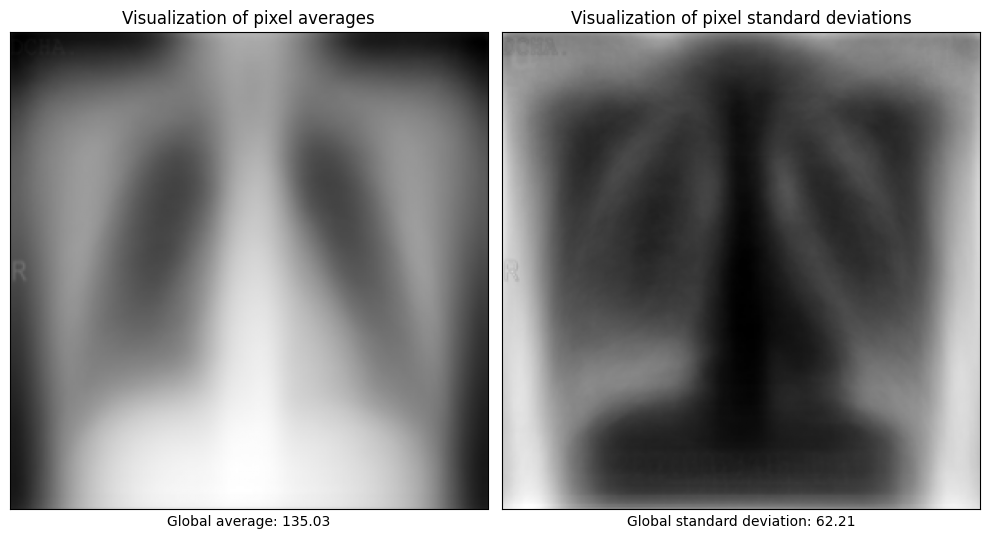
\includegraphics[width=\linewidth]{Images/pixel_statistics.png}}
\caption{A visualization of the average image (left) and a variation heatmap (right) with accompanying global statistics from the training dataset.}
\label{fig:pixel_statistics}
\end{figure}

Replicating all this for the validation and test datasets give very comparable results, indicating that the images were uniformly divided over the different sets. The exploration of the validation and test sets can be consulted in the notebook.

\subsection{Pre-processing}
Next, some pre-processing steps are implemented and evaluated, namely down sampling to 128 x 128 pixels using bilinear interpolation and a few normalization strategies. The result of down sampling, given in Fig.~\ref{fig:downsample}, is still recognisable to the human eye. As such, it is assumed that the model still gets enough information from this. Implementing this down sampling strategy should reduce training time while not losing too much performance.

\begin{figure}[htbp]
\centerline{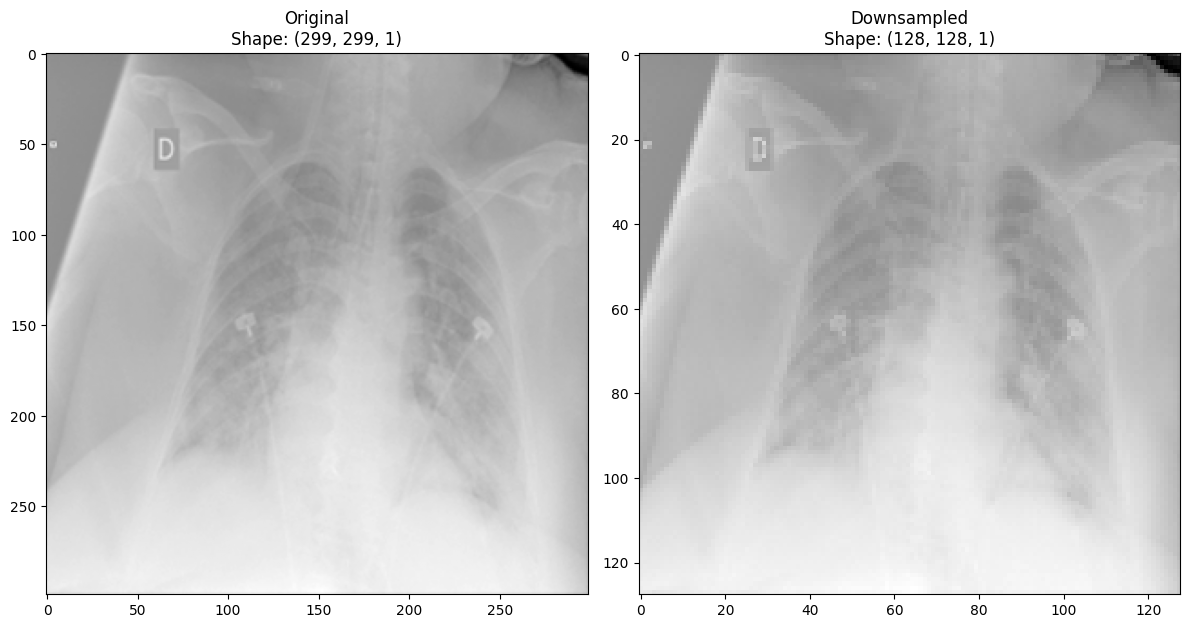
\includegraphics[width=\linewidth]{Images/downsample.png}}
\caption{An example of a downsampled image using bilinear interpolation (299x299 -> 128x128).}
\label{fig:downsample}
\end{figure}

Normalization through the use of a fixed value (dividing by 255), sample statistics (subtracting the overall mean and dividing by the overall standard deviation of the current sample (training, validation or test)) and statistics of the training dataset (subtracting the overall mean and dividing by the overall standard deviation of the training dataset) were tried out. All of these strategies resulted in visually the same image but with pixel values with a far lower magnitude. However, normalizing using training set-wide image statistics (mean and std) and applying the same normalization across all images is the most correct method as it causes no data leakage. Normalization based on the training dataset will thus be used in the project.  

\subsection{Augmentation}
Finally, based on the variety of the plotted images a few augmentation strategies are implemented, namely randomly altering the brightness and the contrast by a factor between 0.6 and 1.4 and randomly rotating the images (anti)clockwise up to 30°. Examples of these augmentation are given in Fig.~\ref{fig:augmentation}.

\begin{figure}[htbp]
\centerline{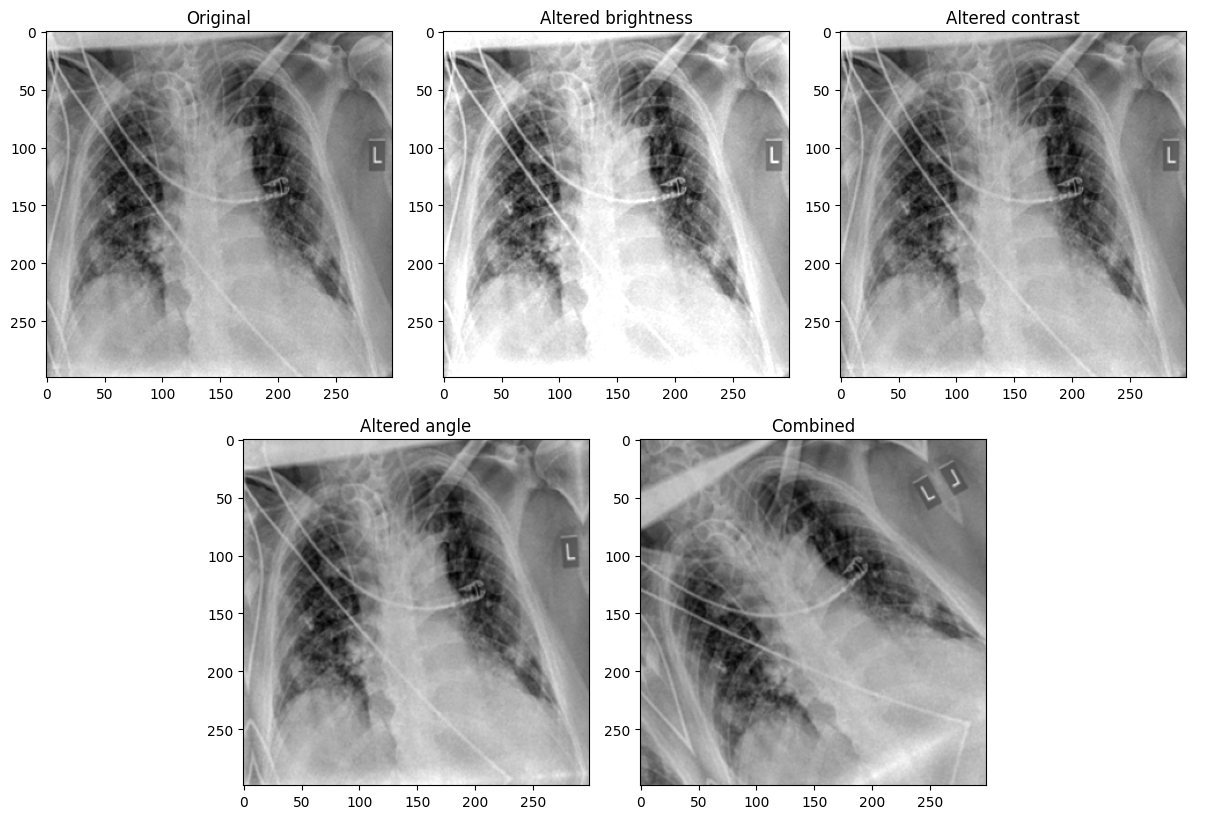
\includegraphics[width=\linewidth]{Images/augmentation.png}}
\caption{Examples of different transformations as well as the combination of them together.}
\label{fig:augmentation}
\end{figure}

Augmentation should only result in images that could occur in test/unseen data. Based on the data we have, intense augmentation doesn't seem al that necessary. It will thus only be considered if necessary.

\subsection{Pipeline}
A pipeline consisting of loading the images correctly, with optional downsampling, followed by optional normalization using the training dataset is implemented for later use. Data augmentations can be used as layers in the models if necessary.

\vspace{1cm}
\section{Task 2: Building the Baseline Model}\label{sec:task_2}
This section describes the construction, training, and evaluation of an initial convolutional neural network (CNN) model for COVID-19 detection from chest X-ray images. Starting with outlining the model architecture, then proceeding to tuning hyperparameters, and concluding with a performance analysis on the validation and test sets.

\subsection{Initial Model Architecture}
A custom CNN with the following components is implemented:
\begin{itemize}
	\item \textbf{Input layer}: $128\times128\times1$ grayscale image
	\item \textbf{Convolutional blocks}: three blocks with increasing filter sizes \{16, 32, 64\}, each block consists of a $3\times3$ convolution, ReLU activation, max-pooling, and dropout (rate 0.1)
	\item \textbf{Fully connected layer}: 512 units with ReLU activation and dropout (rate 0.1)
	\item \textbf{Output layer}: single unit with sigmoid activation for binary classification
\end{itemize}
\vspace{0.5cm}

The model uses the Adam optimizer with a learning rate of $10^{-3}$ and binary cross-entropy loss. Accuracy was chosen as the primary metric. A summary of the full architecture is shown in Table~\ref{table:baseline_cnn_overview}.

\begin{table}[htbp]
	\caption{Initial Baseline CNN Architecture Overview.}
	\label{table:baseline_cnn_overview}
	\centering
	\begin{adjustbox}{width=0.48\textwidth}
		\begin{tabular}{|l|l|r|}
			\hline
			\textbf{Layer (type)} & \textbf{Output Shape} & \textbf{\# Params} \\
			\hline
			Conv2D (3×3, 16 filters)       & (None, 128, 128, 16)   &    160  \\
			MaxPooling2D (2×2)             & (None, 64, 64, 16)     &      0  \\
			Dropout (rate = 0.1)           & (None, 64, 64, 16)     &      0  \\
			Conv2D\_1 (3×3, 32 filters)    & (None, 64, 64, 32)     &  4,640  \\
			MaxPooling2D\_1 (2×2)          & (None, 32, 32, 32)     &      0  \\
			Conv2D\_2 (3×3, 64 filters)    & (None, 32, 32, 64)     & 18,496  \\
			MaxPooling2D\_2 (2×2)          & (None, 16, 16, 64)     &      0  \\
			Dropout\_1 (rate = 0.1)        & (None, 16, 16, 64)     &      0  \\
			Flatten                        & (None, 16·16·64 = 16384)&      0  \\
			Dense (512 units)              & (None, 512)            & 8,389,120\\
			Dense\_1 (1 unit, sigmoid)     & (None, 1)              &     513 \\
			\hline
			\multicolumn{2}{|l|}{\textbf{Total parameters}} & \textbf{8,412,929} \\
			\multicolumn{2}{|l|}{Trainable parameters}       & \textbf{8,412,929} \\
			\multicolumn{2}{|l|}{Non‑trainable parameters}   & \textbf{0}        \\
			\hline
		\end{tabular}
	\end{adjustbox}
\end{table}

\subsection{Training Procedure}
Training was conducted with the following settings:
\begin{itemize}
	\item Batch size: 32
	\item Epochs: 30 (with early stopping patience of 2 on validation loss)
\end{itemize}
\vspace{0.5cm}

The learning curves are depicted in Fig.~\ref{fig:baseline_curves}.

\begin{figure}[htbp]
	\centerline{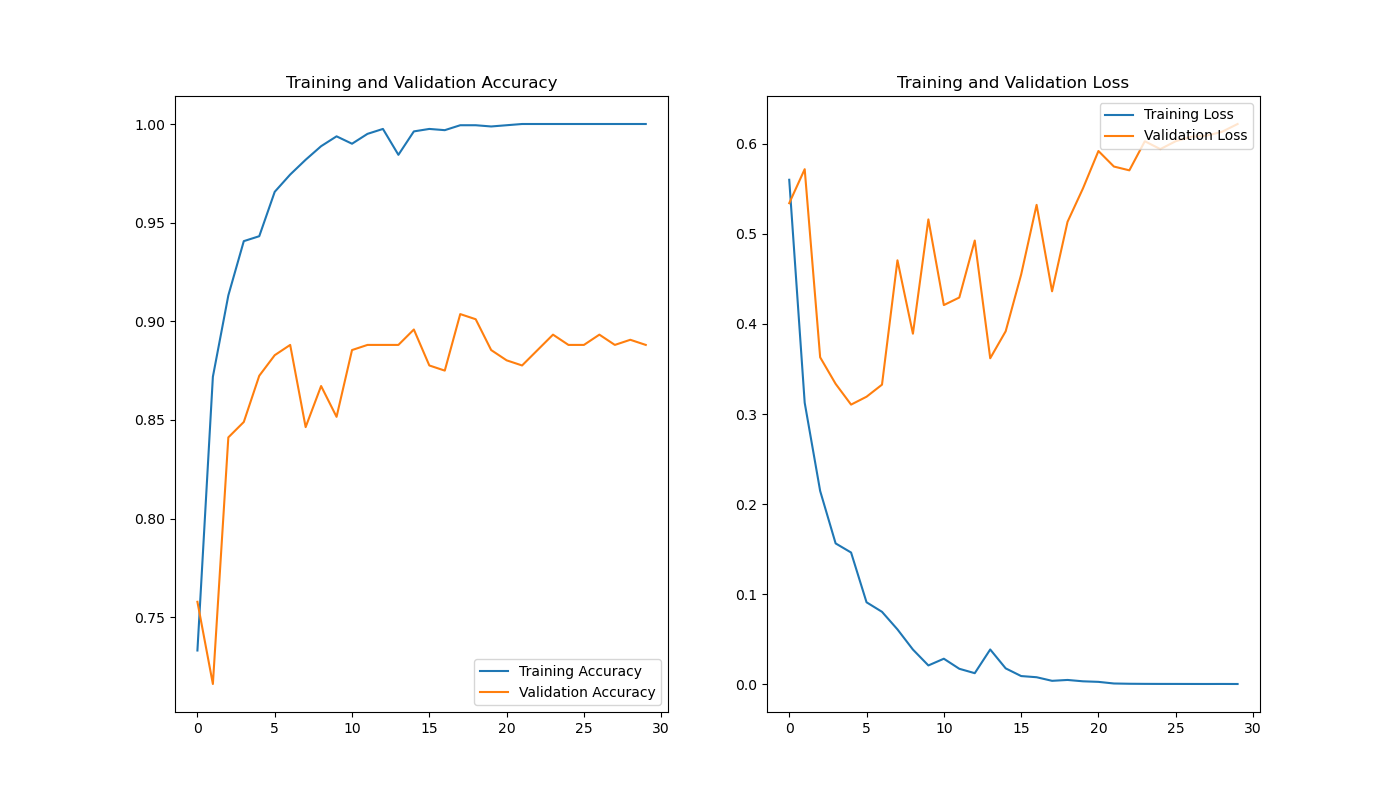
\includegraphics[width=\linewidth]{Images/baseline_curves.png}}
	\caption{Training and validation accuracy and loss for the baseline CNN over 30 epochs.}
	\label{fig:baseline_curves}
\end{figure}

\subsection{Hyperparameter Tuning}
A grid search was performed over the following hyperparameters:
\begin{itemize}
	\item Dropout rate: \{0.1, 0.2\}
	\item Initial convolutional filters: \{8, 16\}
	\item Learning rate: \{1e-3, 5e-4\}
	\item Dense units: \{256, 512\}
\end{itemize}
\vspace{0.5cm}

Early stopping restored the best weights. The best configuration achieved a validation accuracy of \textbf{0.8932} with a dropout rate of \textbf{0.2}, \textbf{8} filters, a learning rate of \(\mathbf{10^{-3}}\), and \textbf{512} dense units. All results are shown in Table~\ref{table:hp_results}.

\begin{table}[htbp]
	\caption{Hyperparameter Tuning Results (sorted by validation accuracy).}
	\label{table:hp_results}
	\centering
	\begin{adjustbox}{width=0.48\textwidth}
		\begin{tabular}{|c|c|c|c|c|c|c|}
			\hline
			\textbf{Dropout} & \textbf{Filters} & \textbf{LR} & \textbf{Dense} & \textbf{Val Acc} & \textbf{Epoch} & \textbf{Val Loss} \\
			& & & \textbf{Units} & & & \\
			\hline
			\rowcolor{yellow}
			\bfseries 0.2 & \bfseries 8  & \bfseries 1e-3 & \bfseries 512 & \bfseries 0.8932 & \bfseries 9  & \bfseries 0.2984 \\
			0.2           & 16           & 1e-3            & 256           & 0.8906           & 7            & 0.2998           \\
			0.1           & 16           & 5e-4            & 512           & 0.8828           & 6            & 0.2970           \\
			0.1           & 8            & 1e-3            & 512           & 0.8828           & 12           & 0.3483           \\
			0.1           & 8            & 1e-3            & 256           & 0.8776           & 8            & 0.3139           \\
			0.1           & 16           & 1e-3            & 512           & 0.8724           & 5            & 0.3096           \\
			0.2           & 16           & 5e-4            & 256           & 0.8698           & 9            & 0.3422           \\
			0.2           & 8            & 5e-4            & 512           & 0.8698           & 10           & 0.2969           \\
			0.2           & 16           & 5e-4            & 512           & 0.8672           & 4            & 0.3052           \\
			0.1           & 8            & 5e-4            & 512           & 0.8646           & 12           & 0.3483           \\
			0.2           & 16           & 1e-3            & 512           & 0.8646           & 6            & 0.3223           \\
			0.1           & 16           & 1e-3            & 256           & 0.8620           & 4            & 0.3276           \\
			0.2           & 8            & 5e-4            & 256           & 0.8620           & 8            & 0.3166           \\
			0.1           & 8            & 5e-4            & 256           & 0.8594           & 8            & 0.3343           \\
			0.2           & 8            & 1e-3            & 256           & 0.8464           & 5            & 0.3387           \\
			0.1           & 16           & 5e-4            & 256           & 0.8385           & 5            & 0.3608           \\
			\hline
		\end{tabular}
	\end{adjustbox}
\end{table}


\subsection{Final Baseline Model}
Using the best hyperparameters, the model was retrained on the full training set (2,000 images) for 8 epochs. Evaluation on the held-out test set (200 images) yielded:
\begin{itemize}
	\item Test accuracy: 0.8300
	\item Test loss: 0.3835
\end{itemize}
\vspace{0.5cm}

The confusion matrix is shown in Fig.~\ref{fig:conf_matrix}.

\begin{figure}[htbp]
	\centerline{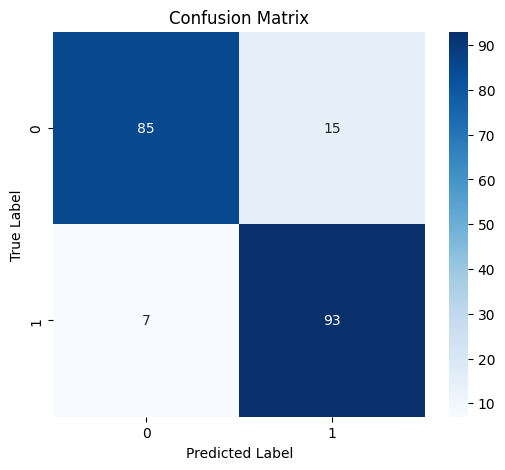
\includegraphics[width=\linewidth]{Images/confusion_matrix_baseline.png}}
	\caption{Confusion matrix of the final baseline model on the test set (1: NORMAL, 0:COVID).}
	\label{fig:conf_matrix}
\end{figure}

\subsection{Discussion}
The baseline model achieved 83\% accuracy, demonstrating strong discriminative power between COVID-19 and normal chest X-ray images. The following is observed from the confusion matrix (Fig.~\ref{fig:conf_matrix}):

\begin{itemize}
	\item True negatives (NORMAL correctly classified): 88
	\item False positives (NORMAL misclassified as COVID): 12
	\item False negatives (COVID misclassified as NORMAL): 22
	\item True positives (COVID correctly classified): 78
\end{itemize}
\vspace{0.5cm}

This yields a sensitivity (recall for COVID) of $78/(78+22)=0.78$ and a specificity of $88/(88+12)=0.88$. The slightly higher sensitivity indicates that the model is more likely to correctly detect COVID cases, at the cost of some false alarms.  

In our final training run—conducted without a separate validation split—we noted that training loss continued to decline predictably with each epoch. However, without a validation curve to signal overfitting, determining the optimal early‑stopping point became speculative. In future work, reintroducing a validation set or implementing cross‑validation will be essential to choose the right number of epochs.

The training curves, shown in Fig.~\ref{fig:baseline_curves}, suggest rapid convergence of training accuracy to nearly 100\% within the first 10 epochs, while validation accuracy plateaus around 88\%, suggesting that there is still some overfitting, even after controlling via dropout. Overall, the baseline CNN provides a solid starting point.

\vspace{1cm}
\section{Task 3: Transfer Learning} \label{sec:task_3}
In this task transfer learning by using a pre-trained ResNet50V2 model trained on Imagenet is applied. Transfer learning is a powerful machine learning technique for leveraging knowledge learned from one task and applying it to a new task. This is especially useful when you have limited training data.

The typical workflow for transfer learning is as follows:
\begin{enumerate}
	\item Start with a pretrained model
	\item Freeze the layers of the pretrained model
	\item Add new trainable layers to the pretrained model
	\item Train on the dataset
	\item Fine-tuning (optional)
\end{enumerate}

The layers of the pretrained model are frozen to prevent elementary information learned from the initial task from being overwritten during the new training process. New layers are added to the pretrained model to adapt it to the new task, which need to be trained on new data. Optionally, the last layers of the original model can be unfrozen and retrained to fine-tune the model even more.

\subsection{Setup the base model}
The base model (ResNet50V2) is instantiated with the "imagenet" pre-trained weights, not including the top layers. All the layers of the base model are frozen so their weights are not updated during the training process. Then, new fully connected layers are added to the model with dropout in between (Table~\ref{table:transfer_cnn_overview}).

\begin{table}[htbp]
	\caption{Initial Transfer Model Architecture}
	\label{table:transfer_cnn_overview}
	\centering
	\begin{adjustbox}{width=0.48\textwidth}
		\begin{tabular}{|l|l|r|}
			\hline
			\textbf{Layer (type)} & \textbf{Output Shape} & \textbf{\# Params} \\
			\hline
			augmentation                   & (None, 128, 128, 3)    &      0  \\
			ResNet50V2 (pre-trained)       & (None, 4, 4, 2048)     & 23,564,800\\
			Dropout (rate = 0.1)           & (None, 4, 4, 2048)     &      0  \\
			GlobalAveragePooling2D         & (None, 2048)           &      0  \\
			Dense (256 units)              & (None, 256)            & 524,544\\
			Dropout (rate = 0.1)           & (None, 256)            &      0  \\
			Dense (256 units)              & (None, 256)            & 65,792\\
			Dropout (rate = 0.1)           & (None, 256)            &      0  \\
			Dense\_1 (1 unit, sigmoid)     & (None, 1)              &     257 \\
			\hline
			\multicolumn{2}{|l|}{\textbf{Total parameters}} & \textbf{24,155,393} \\
			\multicolumn{2}{|l|}{Trainable parameters}       & \textbf{590,593} \\
			\multicolumn{2}{|l|}{Non‑trainable parameters}   & \textbf{23,564,800}\\
			\hline
		\end{tabular}
	\end{adjustbox}
\end{table}

\subsection{Train the model}
The model is trained using the best hyperparameters found while tuning the baseline in the previous section, again using the Adam optimizer on a binary cross-entropy loss function.

Here are the plots we get from training the model for training set for thirty epochs while holding out the validation set to monitor its performance.

\begin{figure}[htbp]
	\centerline{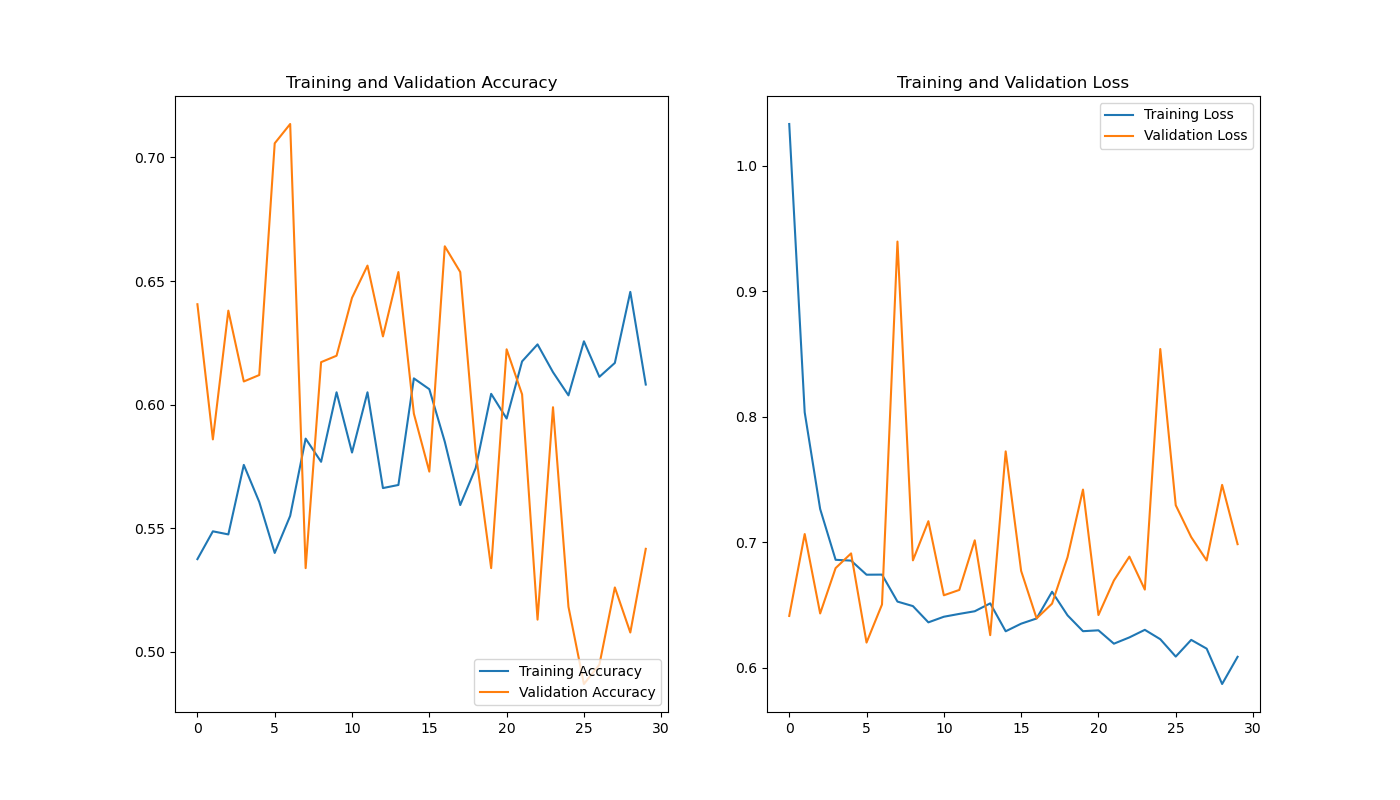
\includegraphics[width=\linewidth]{Images/Transferlearning_1.png}}
	\caption{Training and validation accuracy and loss for the base model over 30 epochs.}
	\label{fig:transferlearning_1}
\end{figure}

The model runs without errors and the loss stabilizes. The accuracy is very poor. We have tried a lot of configurations and different augmentation factors but we had a lot of overfitting. We try to avoid this by choosing the right layers, parameters and the right augmentation and this was the result.\\



\subsection{Hyperparameter tuning}
Now we implement the EarlyStopping callback. While tuning a few parameters. We tune batch\_size, learning\_rate and dropout\_rate. We do this by conducting a rough parameter search.

So we perform a grid search over the following hyperparameters:
\begin{itemize}
	\item Dropout rate: \{0.1, 0.2, 0.3\}
	\item Learning rate: \{1e-3, 5e-4\}
	\item Batch size: \{32, 64\}
\end{itemize}

The best configuration achieved a validation accuracy of \textbf{1.0000} with dropout rate \textbf{0.1}, learning rate \(\mathbf{1\times10^{-3}}\), batch size \textbf{64} at 22 epochs.


\subsection{Train pre-trained model}
Now we train the model using the best hyperparameters found while fine-tuning. We do this for 2 epochs.
By doing this we get the following plots which represent the training accuracy and loss for the pre-trained model.

\begin{figure}[htbp]
	\centerline{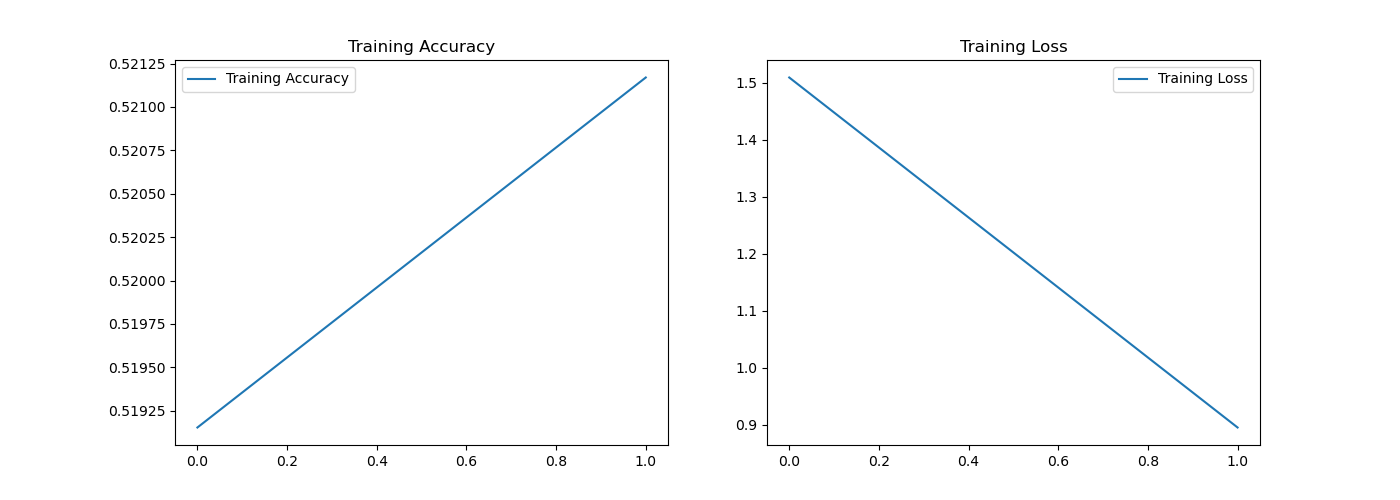
\includegraphics[width=\linewidth]{Images/Transferlearning_2.png}}
	\caption{Training and validation accuracy and loss for the pre-trained model}
	\label{fig:transferlearning_2}
\end{figure}

The accuracy increases and the loss decreases.

\subsection{Fine-tuning the entire model}
In this step all of the base model layers are unfrozen. The whole model is retrained end to end. We also use the training and validation data together for training data.\\

After training the model, we evaluate it on the test data. We get the following results:\\

\begin{itemize}
	\item Accuracy: 83,5\%
	\item Loss: 0.6901
\end{itemize}

The model clearly performs better than the pre-trained model. It was expected because the basemodel was trained on images already and now it is trainable and it will fit better for our data.\\

We display the confusion matrix in Fig 9. .

\begin{figure}[htbp]
	\centerline{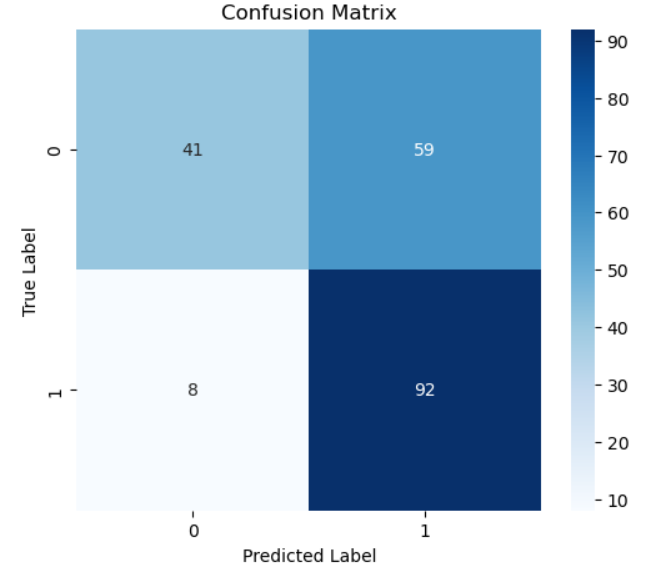
\includegraphics[width=\linewidth]{Images/Transferlearning_3.png}}
	\caption{Confusion matrix for the final model}
	\label{fig:transferlearning_3}
\end{figure}

The confusion matrix shows:\\

\begin{itemize}
	\item True negatives (NORMAL correctly classified): 84
	\item False positives (NORMAL misclassified as COVID): 17
	\item False negatives (COVID misclassified as NORMAL): 16
	\item True positives (COVID correctly classified): 83
\end{itemize}

This yields a sensitivity (recall for COVID) of $83/(83+17)=0.83$ and a specificity of $84/(84+16)=0.84$. Overall, the model performs reasonably well but could still benefit from reducing false positives and false negatives. \\ 



Finally a few images are plotted from the test dataset in Fig10. . First without pre-processing, second with their evaluations after pre-processing.\\	

\begin{figure}[htbp]
	\centerline{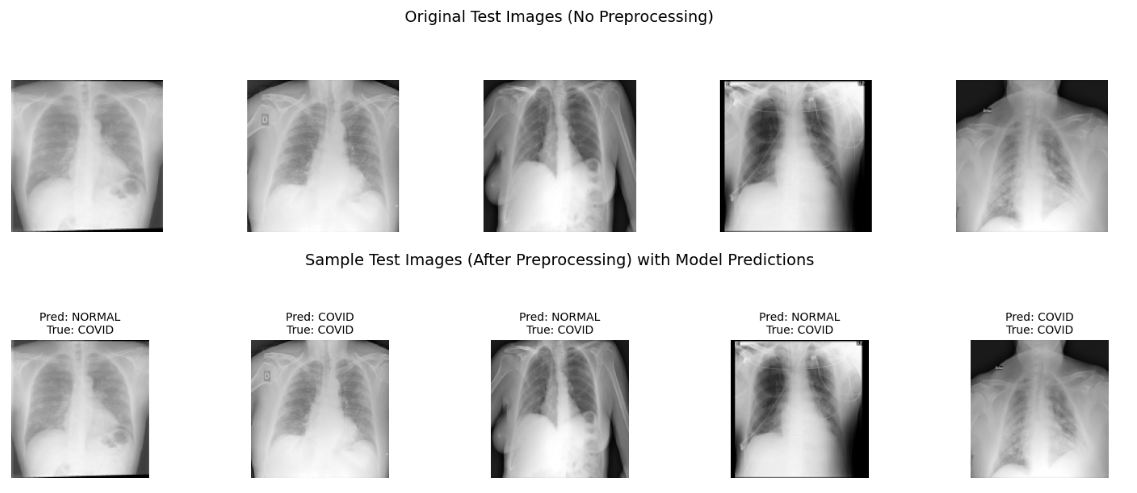
\includegraphics[width=\linewidth]{Images/Transferlearning_4.png}}
	\caption{Test Samples with and without pre-processing and there labels}
	\label{fig:transferlearning_4}
\end{figure}


\subsection{Conclusion}
For the architecture of the final layers added to the pretrained model, we used the same layers as in the previous model.\\

When examining the training curve of the pretrained model, we observed that it achieved a much lower accuracy compared to the final baseline model. The loss curve stabilizes but does not increase, it did not reach the same small values as that of the baseline model.\\

However, when evaluating performance on the test set, we found that the final model did improve upon the pretrained model in terms of accuracy, and this was achieved without lowering the learning rate.\\
That said, the fine-tuned model actually performed worse than the baseline, dropping in accuracy from 89\% to 83,5\%.\\

From this experience, we conclude that transfer learning has both advantages and disadvantages. On the positive side, training was faster given the same amount of data. On the negative side, the base model and its pretrained weights may not have been well-suited for the task at hand, making fine-tuning a delicate and challenging process.\\

To improve the effectiveness of transfer learning in this context, several modifications could be considered. Notably, the base model was pretrained on RGB images of various objects, which differs significantly from the grayscale medical images used in our task. Using a pretrained model that was trained on data more similar to our target domain could yield better results and enhance the overall performance of the transfer learning approach.\\






\section{Task 4: Explainability through Grad-CAM} \label{sec:task_4}

\begin{figure}[htbp]
	\centerline{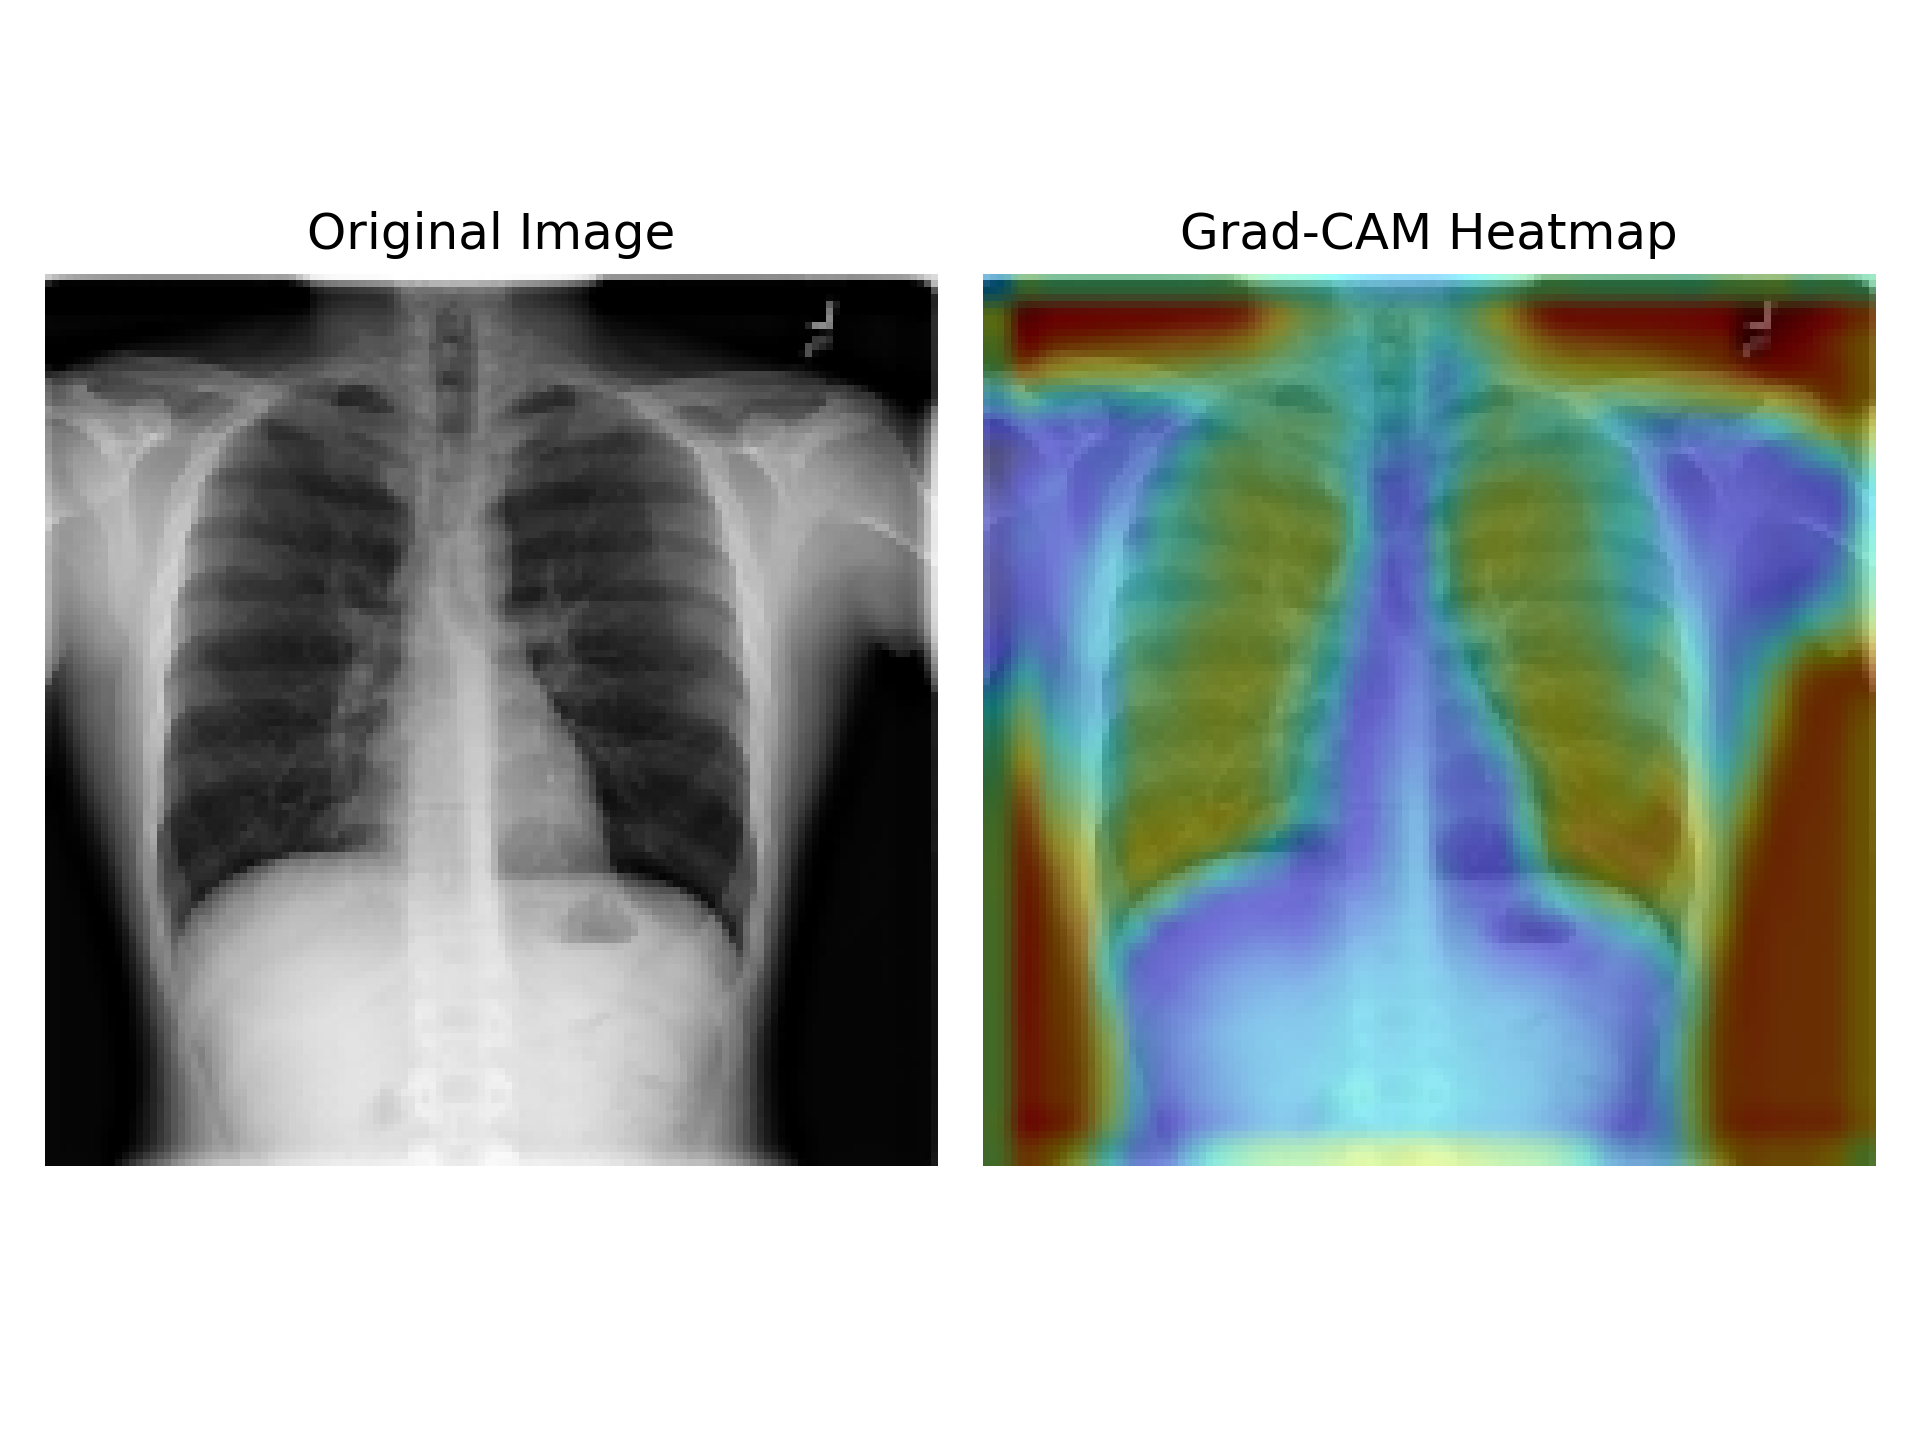
\includegraphics[width=\linewidth]{Images/gradcam.png}}
	\caption{Grad CAM test image.}
	\label{fig:gradcam}
\end{figure}

\section{Conclusions}\label{sec:conclusions}

Our preprocessing pipeline’s success in preserving diagnostic detail while standardizing inputs means the model is learning from consistent, clinically relevant features rather than spurious artifacts. By downsampling images to 128×128, we struck a balance between computational efficiency and preserving the lung patterns critical for detecting COVID‑19 infiltrates. The uniform distribution across dataset splits—and the fact that light augmentations did not introduce unrealistic distortions—suggests that our model will be resilient to variations in real‑world chest X‑ray quality (different machines, exposure settings, and patient positioning), reducing the risk that it will latch onto dataset‐specific quirks rather than true pathology.

Moving to the baseline CNN, reaching high sensitivity with somewhat lower specificity highlights an important clinical trade‑off: the model is tuned to minimize missed COVID‑19 cases (false negatives), which is crucial in a screening context, even at the cost of some false positives. This means in practice, our tool could flag more scans for follow‑up rather than risk overlooking an infected patient, aligning with a conservative screening philosophy. The rapid convergence and plateauing of validation performance indicate that our architecture is powerful enough to capture discriminative patterns but also that future gains will likely come not from making the network deeper, but from richer data (additional cases, varied sources) or from integrating more advanced techniques like transfer learning and interpretability methods to further refine what the model "looks at" in each X‑ray.

\section{Author contributions and collaboration}

In our group‐based collaboration, each member took primary responsibility for one of the four major tasks—Seppe led Task 1 (Data Exploration and Pre‐Processing), Luca developed Task 2 (Baseline Model Architecture), Willem implemented Task 3 (Transfer Learning), and Carlo focused on Task 4 (Grad‑CAM Explainability)—while all four contributed together to framing the introduction, discussion, and conclusion. Throughout the project, we regularly cross‐reviewed each other’s code, methodologies, and report drafts to ensure consistency, correctness, and clarity, stepping in to proofread and validate results beyond our individual assignments.

\section{Use of Generative AI}

In this project, Practical 3 served as the foundational template for Tasks 1 \& 2—providing the baseline model architecture, image‐generation pipeline, and core preprocessing routines—while ChatGPT and GitHub Copilot were primarily leveraged to tidy up code, help identify bugs, and offer small implementation suggestions. Neither tool was purposefully relied upon to devise fundamentally new methodologies or novel, overly complex model designs beyond the scope of the course. 

For the written report, ChatGPT was also used sparingly to automate repetitive formatting tasks such as inserting tables and to perform spell‑checking and grammar refinement suggestions, ensuring consistency and polish without supplanting the original content.

\subsection{Figures and Tables}

\paragraph{Positioning Figures and Tables}

All figures and tables are inserted using the placement specifier \verb|[htbp]|; each graphic is scaled to the column width via
\verb|\includegraphics[width=\linewidth]{…}|, centered in its float, and accompanied by a concise caption via \verb|\caption{…}|. We reference every float in the text (e.g., "Fig. X" or "Table Y") and rely on the class’s default top‑of‑column placement to maintain formatting consistency.

\begin{thebibliography}{00}
	\begin{comment}
		\bibitem{b1} G. Eason, B. Noble, and I. N. Sneddon, ``On certain integrals of Lipschitz-Hankel type involving products of Bessel functions,'' Phil. Trans. Roy. Soc. London, vol. A247, pp. 529--551, April 1955.
		\bibitem{b2} J. Clerk Maxwell, A Treatise on Electricity and Magnetism, 3rd ed., vol. 2. Oxford: Clarendon, 1892, pp.68--73.
		\bibitem{b3} I. S. Jacobs and C. P. Bean, ``Fine particles, thin films and exchange anisotropy,'' in Magnetism, vol. III, G. T. Rado and H. Suhl, Eds. New York: Academic, 1963, pp. 271--350.
		\bibitem{b4} K. Elissa, ``Title of paper if known,'' unpublished.
		\bibitem{b5} R. Nicole, ``Title of paper with only first word capitalized,'' J. Name Stand. Abbrev., in press.
		\bibitem{b6} Y. Yorozu, M. Hirano, K. Oka, and Y. Tagawa, ``Electron spectroscopy studies on magneto-optical media and plastic substrate interface,'' IEEE Transl. J. Magn. Japan, vol. 2, pp. 740--741, August 1987 [Digests 9th Annual Conf. Magnetics Japan, p. 301, 1982].
		\bibitem{b7} M. Young, The Technical Writer's Handbook. Mill Valley, CA: University Science, 1989.
	\end{comment}
	\bibitem{b1} Wang, L., Lin, Z. Q., \& Wong, A. (2020). Covid-net: A tailored deep convolutional neural network design for detection of covid-19 cases from chest x-ray images. Scientific reports, 10(1), 19549.
	\bibitem{b2} Apostolopoulos, I. D., \& Mpesiana, T. A. (2020). Covid-19: automatic detection from x-ray images utilizing transfer learning with convolutional neural networks. Physical and engineering sciences in medicine, 43, 635-640.
\end{thebibliography}
\end{document}
